\chapter{Limits and Continuity}


\section{Some Topology}
\begin{df}
Let $\vector{a}\in\reals^n$ and let $\varepsilon > 0$. An \negrito{open
ball} centered at $\vector{a}$ of radius $\varepsilon$ is the set
$$ \ball{\vector{a}}{\varepsilon} = \{\vector{x}\in\reals^n: \norm{\vector{x}-\vector{a}} <
\varepsilon\}.
$$An \negrito{open box} is a Cartesian product of open intervals
$$ ]a_1; b_1[\times  ]a_2; b_2[\times  \cdots \times   ]a_{n-1}; b_{n-1}[\times  ]a_n; b_n[,$$
where the $a_k, b_k$ are real numbers.
\end{df}

The set $$ \ball{\vector{a}}{\varepsilon} = \{\vector{x}\in\reals^n: \norm{\vector{x}-\vector{a}} <
\varepsilon\}.
$$ are also called the \negrito{$\varepsilon$-neighborhood} of the point $a$.



\vspace{3cm}
\begin{figure}[htpb]
\begin{minipage}{7cm}
\centering \psset{unit=0.7pc}
\psaxes[linewidth=2pt,labels=none,ticks=none]{->}(0,0)(-1,-1)(8,8)
\pstGeonode[PointName=none](4,4){A}(0,0){O}
\pstTranslation[DistCoef=.35,PointName=none,PointSymbol=none]{O}{A}{A}[B]
\pscircle*[linecolor=YellowGreen](A){2}\pscircle[linestyle=dashed,linewidth=2pt](A){2}
\uput[d](A){\tiny{$(a_1,a_2)$}}
\ncline{->}{A}{B}\aput{:U}{$\varepsilon$}
\vspace{1cm}\footnotesize\hangcaption{Open ball in $\reals^2$.}
\label{fig:open-ball-r2}
\end{minipage}
\hfill
\begin{minipage}{7cm}
\centering \psset{unit=0.7pc}
\psaxes[linewidth=2pt,labels=none,ticks=none]{->}(0,0)(-1,-1)(8,8)
\pstGeonode[PointName=none](1,3){A}(8,3){B}(8,6){C}(1,6){D}
\pspolygon*[linecolor=RoyalBlue](A)(B)(C)(D)
\pstLineAB[linestyle=dashed,linewidth=2pt]{A}{B}\bput{:U}{$b_1-a_1$}
\ncline[linestyle=dashed,linewidth=2pt]{B}{C}\bput{:U}{$b_2-a_2$}
\ncline[linestyle=dashed,linewidth=2pt]{C}{D}
\ncline[linestyle=dashed,linewidth=2pt]{D}{A}
\pstMiddleAB[PointName=none]{A}{C}{M}
\vspace{1cm}\footnotesize\hangcaption{Open rectangle in $\reals^2$.}
\label{fig:open-box-r2}
\end{minipage}
\end{figure}

\vspace{2.5cm}
\begin{figure}[htpb]
\begin{minipage}{7cm}
\centering \psset{unit=0.7pc}
 \psset{unit=2.8pc}
\pstThreeDCoor[xMin=0,xMax=2,yMin=0,yMax=2,zMin=0,zMax=2]%
\pstGeonode[PointName=none](1,.5){A}(0,0){O}
\pstTranslation[DistCoef=.9,PointName=none,PointSymbol=none]{O}{A}{A}[B]
\pstCircleOA[linestyle=dashed,linewidth=2pt,
Radius=\pstDistVal{1},linecolor=red]{A}{}\pstLineAB[arrows={->}]{A}{B}
\aput{:U}{$\varepsilon$} \uput[r](A){\tiny$(a_1,a_2,a_3)$}
\psellipse[linestyle=dashed,linewidth=1.2pt](A)(1,.25)
\vspace{1cm}\footnotesize\hangcaption{Open ball in $\reals^3$.}
\label{fig:open-ball-r3}
\end{minipage}
\hfill
\begin{minipage}{7cm}
\centering \psset{unit=2.8pc}
\pstThreeDCoor[xMin=0,xMax=2,yMin=0,yMax=2,zMin=0,zMax=2]%
\pstThreeDBox[fillstyle=gradient,linewidth=2pt,linestyle=dashed](1,1,2)(1,0,0)(0,2,0)(0,0,.5)
\vspace{1cm}\footnotesize\hangcaption{Open box in $\reals^3$.}
\label{fig:open-box-r3}
\end{minipage}
\end{figure}



\begin{exa}
An open ball in $\reals$ is an open interval, an open ball in
$\reals^2$ is an open disk  and
an open ball in $\reals^3$ is an open sphere. An open box in $\reals$ is an open
interval, an open box in $\reals^2$ is a rectangle without its
boundary  and an  open box in
$\reals^3$ is a box without its boundary.
\end{exa}
\begin{df}
A set $A \subseteq \reals^n$ is said to be \negrito{open} if
for every point belonging to it we can surround the point by a
sufficiently small open ball so that this balls lies completely
within the set. That is, $\forall\vector{a}\in A \ \
\exists \varepsilon > 0$ such that $\ball{\vector{a}}{\varepsilon}
\subseteq A$.
\end{df}

\begin{figure}[h]
\centering
\scalebox{0.7}{
 \tikz\foreach \i in {0,...,0}\foreach \j in {0,...,2}
  \draw [blue!50!black, dashed, ultra thick, shift={(\j*6,\i*6)}] 
    plot [smooth cycle, tension=1, domain=0:320, samples=12] (\x:{2+rand/2});
    }
    \caption{Open Sets}
\end{figure}



\begin{exa}
The open interval $]-1; 1[$ is open in $\reals$. The interval $]-1;
1]$ is not open, however, as no interval centred at $1$ is totally
contained in $]-1; 1]$.
\end{exa}\begin{exa}
The region  $]-1; 1[\times ]0; +\infty[$ is open in $\reals^2$.
\end{exa}
\begin{exa}
The ellipsoidal region $\left\{(x,y)\in\reals^2: x^2 + 4y^2 <
4\right\}$ is open in $\reals^2$.
\end{exa}
The reader will recognize that open boxes, open ellipsoids and their
unions and finite intersections are open sets in $\reals^n$.
\begin{df}
A set $F \subseteq \reals^n$ is said to be \negrito{closed}
in $\reals^n$ if its complement $\reals^n \setminus F$
is open.
\end{df}
\begin{exa}
The closed interval $[-1; 1]$ is closed in $\reals$, as its
complement, $\reals \setminus [-1;1] = ]-\infty; -1[\cup ]1;
+\infty[$ is open in $\reals$. The interval $]-1; 1]$ is neither
open nor closed in $\reals$, however.
\end{exa}\begin{exa}
The region  $[-1; 1]\times [0; +\infty[\times [0; 2]$ is closed in
$\reals^3$.
\end{exa}

\begin{lemma}\label{thmtype:5.1.12}
If $\vector{x}_1$ and $\vector{x}_2$ are in $S_r(\vector{x}_0)$ for some $r>0$,
then so is every point on
the line segment from $\vector{x}_1$ to $\vector{x}_2.$
\end{lemma}

\begin{proof}
The line segment is given by
$$
\vector{x}=t\vector{x}_2+(1-t)\vector{x}_1,\quad 0<t<1.
$$
Suppose that $r>0$. If
$$
|\vector{x}_1-\vector{x}_0|<r,\quad |\vector{x}_2-\vector{x}_0|<r,
$$
and $0<t<1$, then
\begin{eqnarray*}
|\vector{x}-\vector{x}_0|=|t\vector{x}_2+(1-t)\vector{x}_1-t\vector{x}_0-(1-t)\vector{x}_0|\\
=|t(\vector{x}_2-\vector{x}_0)+(1-t)\vector{x}_1-\vector{x}_0)|\\
\le  t|\vector{x}_2-\vector{x}_0|+(1-t)|\vector{x}_1-\vector{x}_0|\\
< tr+(1-t)r=r.
\end{eqnarray*}
\end{proof}


\begin{definition}\label{thmtype:5.1.13}
A sequence of points $\{\vector{x}_r\}$ in $  \bbR^n$
\negrito{converges to the limit\/} $\overline{\vector{x}}$ if
$$
\lim_{r\to\infty} |\vector{x}_r-\overline{\vector{x}}|=0.
$$
In this case we write
$$
\lim\limits_{r\to\infty}\vector{x}_r=\overline{\vector{x}}.
$$
\end{definition}



The next two theorems follow from this, the definition of
distance in $  \bbR^n$, and what we already know about convergence
in $  \bbR$. 
\begin{thm}\label{thmtype:5.1.14}
Let
$$
\overline{\vector{x}}=(\overline{x}_1,\overline{x}_2,
\dots,\overline{x}_n)
\mbox{\quad and\quad}\vector{x}_r=(x_{1r}, x_{2r}, \dots, x_{nr}),\quad
r\ge1.
$$
Then $\lim\limits_{r\to\infty}\vector{x}_r=\overline{\vector{x}}$ if and only if
$$
\lim\limits_{r\to\infty}x_{ir}=\overline{x}_i,\quad 1\le i\le n;
$$
that is$,$ a sequence $\{\vector{x}_r\}$ of points in $  \bbR^n$
converges
to a limit $\overline{\vector{x}}$ if and only if the sequences of
components of $\{\vector{x}_r\}$ converge to the respective
components of
$\overline{\vector{x}}.$
\end{thm}




\begin{thm} [Cauchy's Convergence Criterion]\label{thmtype:5.1.15}
A sequence $\{\vector{x}_r\}$  in $  \bbR^n$ converges if and
only if for each $\varepsilon>0$ there is an integer $K$ such that
$$
\norm{\vector{x}_r-\vector{x}_s}<\varepsilon\mbox{\quad if\quad} r,s\ge K.
$$
\end{thm}







\begin{df}\label{thmtype:1.3.4} Let $S$ be a subset of ${\bbR}$. Then
\begin{enumerate}
\item % (a)
 $x_0$ is a \negrito{limit point\/}
of $S$ if every deleted neighborhood of $x_0$ contains a point of~$S$.


\item % (b)
$x_0$ is a \negrito{boundary point\/} of $S$ if every neighborhood
of $x_0$ contains at least one point in $S$ and one not in $S$. The set of
boundary points of $S$ is the \negrito{boundary\/} of $S$, denoted by $\partial
S$. The \negrito{closure\/} of $S$, denoted by $\overline{S}$, is
$\overline{S}=S\cup \partial S$.


\item % (c)
$x_0$ is an \negrito{isolated point} of $S$ if $x_0\in S$
 and there is a neighborhood of $x_0$ that contains no other point of
$S$.

\item % (d)
$x_0$ is \negrito{exterior} to $S$ if $x_0$ is in the interior of $S^c$. The
collection of such points is the \negrito{exterior\/} of $S$.
\end{enumerate}
\end{df}

\enlargethispage{\baselineskip}
\begin{exa}\label{example:1.3.7}  Let
$S=(-\infty,-1]\cup (1,2)\cup
\{3\}$. Then
  \begin{enumerate}
\item % (a)
The set of limit points of $S$ is $(-\infty,-1]\cup
[1,2]$.
\item % (b)
$\partial S=\{-1,1,2,3\}$ and $\overline{S}=
(-\infty,-1]\cup [1,2]\cup\{3\}$.
\item % (c)
 $3$ is the only isolated point
of $S$.
\item % (d)
 The exterior of $S$ is $(-1,1)\cup (2,3)\cup (3,\infty)$.
\end{enumerate}
\end{exa}

\begin{exa}\label{example:1.3.8} For $n\ge1$, let
$$
I_n=\left[\frac{1}{2n+1}, \frac{1}{2n}\right]\mbox{\quad and\quad}
S=
\bigcup^\infty_{n=1} I_n.
$$
Then
\begin{enumerate}
\item % (a)
The set of limit points of $S$ is $S\cup\{0\}$.
\item % (b)
$\partial S=
\{x|x=0 \mbox{ or } x=1/n\ (n\ge2)\}$ and
$\overline{S}=S\cup\{0\}$.
\item % (c)
 $S$ has no isolated points.
\item % (d)
 The exterior of $S$ is
\end{enumerate}
$$
(-\infty,0)\cup\left[\bigcup^\infty_{n=1}\left(\frac{1}{2n+2},\frac{1}
{2n+1}\right)\right]\cup\left(\frac{1}{2},\infty\right).
$$
\end{exa}

\begin{exa}\label{example:1.3.9}
Let $S$ be the set of rational numbers. Since every interval contains
a rational number, every real
number is a limit point of $S$; thus, $\overline{S}=\bbR$. Since
every interval also contains an irrational number, every real number is a
boundary
point of $S$; thus $\partial S=\bbR$.
 The interior and exterior of $S$ are both empty, and $S$
has no isolated points.
$S$ is neither open nor closed.
\end{exa}


The next theorem says that $S$ is closed if and only if $S=\overline{S}$
(Exercise~\ref{exerclosed}).

\begin{thm}\label{thmtype:1.3.5}   A set $S$ is closed if and only if
no point of $S^c$ is a limit point of~$S.$
\end{thm}

\begin{proof}
Suppose that $S$ is closed and $x_0\in S^c$. Since $S^c$ is open,
there is a neighborhood of $x_0$ that is contained in $S^c$ and
therefore contains no points of $S$. Hence, $x_0$ cannot be a limit
point of $S$. For the converse, if no point of $S^c$ is a limit point
of $S$ then every point in $S^c$ must have a neighborhood contained
in $S^c$. Therefore, $S^c$ is open and $S$ is closed.
\end{proof}

Theorem~\ref{thmtype:1.3.5} is usually stated as follows.

\begin{corollary}\label{thmtype:1.3.6}  A set is closed if and only if it
contains all its limit points$.$
\end{corollary}



A \negrito{polygonal curve} $P$ is a curve specified by a sequence of points 
$(A_{1},A_{2},\dots ,A_{n})$ called its vertices. The curve itself consists of 
the line segments connecting the consecutive vertices. 

\begin{figure}[h]
\centering

\begin{tikzpicture}
% \draw [gray]  (0,0) -- (1,1) -- (3,1) -- (1,0)  -- (2,-1) -- cycle;
% \draw [red] plot [smooth cycle] coordinates {(0,0) (1,1) (3,1) (1,0) (2,-1)};

\draw [gray, xshift=4cm]  (0,0) -- (1,1.6) -- (1.7,1.7)--(2,0.4) ;
\draw[dotted,gray, xshift=4cm] (2,0.4) -- (3,1);
\draw [gray, xshift=4cm]   (3,1)--(4,0);
% \draw [cyan, xshift=4cm] plot [smooth, tension=2] coordinates { (0,0) (1,1) (2,-2) (3,0)};
      \node [above, xshift=4cm] at (0,0.1) {\small $A_1$};
      \node [above, xshift=4cm] at (1,1.6) {\small $A_2$};
        \node [above, xshift=4cm] at (1.7,1.7) {\small $A_3$};
       \node [above, xshift=4cm] at (4.2,0) {\small $A_n$};
\end{tikzpicture}
\caption{Polygonal curve}
\end{figure}


\begin{df}
A \negrito{domain}  is a  path connected open set. A path connected set $D$ means that 
any 
two points of this set can be connected by a polygonal curve lying within
$D$.  
\end{df}




\begin{df}
A \negrito{simply connected domain} is a path-connected domain where one can continuously shrink any simple closed curve into a point while remaining in the domain.
\end{df}

  Equivalently a pathwise-connected domain  $U \subseteq \bbR^3$ is called \negrito{simply connected} if for every simple closed curve $\Gamma \subseteq U$, there exists a surface $\Sigma \subseteq U$ whose boundary is exactly the curve $\Gamma$.



\begin{figure}[h]
 \centering
 \subfloat[][Simply connected domain]{
 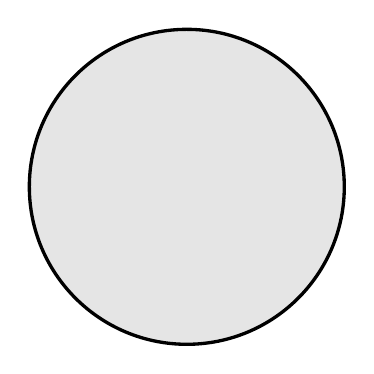
\begin{tikzpicture}
  \usetikzlibrary{arrows}
  \filldraw [black,line width=1.2pt,fill=black!10] (0:0) circle (2);
  %\filldraw [black,line width=1.2pt,fill=white] (0:0) circle (0.5);
%   \node [above right] at (1.5,1.5) {\small $\ssub{\Gamma}{1}$};
  %\node [above] at (0,0.5) {\small $\ssub{\Gamma}{2}$};
%   \node at (0,1.35) {\small $\ssub{R}{1}$};
  %\node at (0,-1.35) {\small $\ssub{R}{2}$};
  %\node [rotate=45] at (-0.3536,0.3536) {\Large $\blacktriangleright$};
  %\node [rotate=45] at (0.3536,-0.3536) {\Large $\blacktriangleleft$};
%   \node [rotate=-45] at (1.4142,1.4142) {\Large $\blacktriangleleft$};
%    \node [rotate=-45] at (-1.4142,-1.4142) {\Large $\blacktriangleright$};
%   \draw [dashed] (0.5,0) -- (2,0);
%   \draw [dashed] (-0.5,0) -- (-2,0);
%   \draw [-latex] (1.05,0.15) -- (1.45,0.15);
%   \draw [latex-] (1.05,-0.15) -- (1.45,-0.15);
%   \draw [-latex] (-1.45,0.15) -- (-1.05,0.15);
%   \draw [latex-] (-1.45,-0.15) -- (-1.05,-0.15);
 \end{tikzpicture}}
 \qquad\qquad
 \subfloat[][Non-simply connected domain]{
 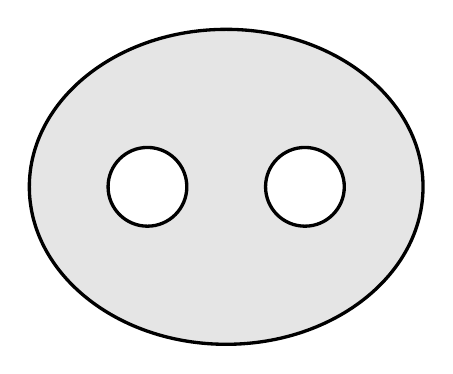
\begin{tikzpicture}
  \usetikzlibrary{arrows}
  \filldraw [black,line width=1.2pt,fill=black!10] (0,0) ellipse (2.5 and 2);
  \filldraw [black,line width=1.2pt,fill=white] (-1,0) circle (0.5);
  \filldraw [black,line width=1.2pt,fill=white] (1,0) circle (0.5);
%   \node [above right] at (1.5,1.6) {\small $\ssub{\Gamma}{1}$};
%   \node [above] at (1,0.5) {\small $\ssub{\Gamma}{2}$};
%   \node [above] at (-1,0.5) {\small $\ssub{\Gamma}{3}$};
%   \node at (0,1.35) {\small $\ssub{R}{1}$};
%   \node at (0,-1.35) {\small $\ssub{R}{2}$};
%    \node [rotate=45] at (-1.3536,0.3536) {\Large $\blacktriangleright$};
%    \node [rotate=45] at (0.6464,0.3536) {\Large $\blacktriangleright$};
%    \node [rotate=45] at (-0.6464,-0.3536) {\Large $\blacktriangleleft$};
%    \node [rotate=45] at (1.3536,-0.3536) {\Large $\blacktriangleleft$};
%    \node [rotate=-31] at (1.5,1.6) {\Large $\blacktriangleleft$};
%    \node [rotate=-31] at (-1.5,-1.6) {\Large $\blacktriangleright$};
%   \draw [dashed] (2.5,0) -- (1.5,0);
%   \draw [dashed] (0.5,0) -- (-0.5,0);
%   \draw [dashed] (-1.5,0) -- (-2.5,0);
%   \draw [-latex] (1.8,0.15) -- (2.2,0.15);
%   \draw [latex-] (1.8,-0.15) -- (2.2,-0.15);
%   \draw [-latex] (-0.2,0.15) -- (0.2,0.15);
%   \draw [latex-] (-0.2,-0.15) -- (0.2,-0.15);
%   \draw [-latex] (-2.2,0.15) -- (-1.8,0.15);
%   \draw [latex-] (-2.2,-0.15) -- (-1.8,-0.15);
 \end{tikzpicture}}
 \qquad\qquad
  \qquad\qquad
 \caption[]{\quad Domains}
 \label{fig:multconn}
\end{figure}  



\section*{\psframebox{Exercises}}
\begin{multicols}{2}\columnseprule 1pt \columnsep 25pt\multicoltolerance=900
\begin{problem}
Determine whether the following subsets of $\reals^2$ are open,
closed, or neither, in $\reals^2$.
\begin{enumerate}
\item $A=\{(x,y)\in\reals^2: |x|<1, |y|<1\}$
\item  $B=\{(x,y)\in\reals^2: |x|<1, |y|\leq 1\}$
\item  $C=\{(x,y)\in\reals^2: |x|\leq 1, |y|\leq 1\}$
\item  $D=\{(x,y)\in\reals^2: x^2\leq y \leq x\}$
\item  $E=\{(x,y)\in\reals^2: xy>1\}$
\item  $F=\{(x,y)\in\reals^2: xy\leq 1\}$
\item  $G=\{(x,y)\in\reals^2: |y|\leq 9, x<y^2\}$
\end{enumerate}
\end{problem}
\begin{problem}[Putnam Exam 1969] Let $p(x,y)$ be a polynomial with real
coefficients in the real variables $x$ and $y$, defined over the
entire plane $\reals^2$. What are the possibilities for the image
(range) of $p(x,y)$? \begin{answer} Since polynomials are continuous
functions and the image of a connected set is connected for a
continuous function, the image must be an interval of some sort. If
the image were a finite interval, then $f(x,kx)$ would be bounded
for every constant $k$, and so the image would just be the point
$f(0,0).$ The possibilities are thus
\begin{enumerate}\item  a single point (take for example,
$p(x,y)= 0$), \item  a semi-infinite interval with an endpoint (take
for example $p(x,y) = x^2$ whose image is $[0; +\infty[$),
\item  a semi-infinite interval with no endpoint (take for example
$p(x,y) = (xy - 1)^2 + x^2$ whose image is $]0; +\infty[$),
\item  all real numbers (take for example $p(x,y) =
x$).
\end{enumerate}
\end{answer}
\end{problem}
\begin{problem}[Putnam 1998] Let ${\cal F}$ be a finite collection of
open disks in $\reals^2$ whose union contains a set $E\subseteq
\reals^2$. Shew that there is a pairwise disjoint subcollection
$D_k, k \geq 1$ in ${\cal F}$ such that
$$E\subseteq \bigcup _{j=1} ^n 3D_j.  $$

\end{problem}

\begin{problem}
 A set $S$ is closed if and only if
no point of $S^c$ is a limit point of~$S.$
\label{exerclosed}
\end{problem}


\end{multicols}

\section{Limits}
 We will start
with the notion of {\em limit}.



\begin{df}
A function $f:\reals^n \rightarrow \reals^m$ is said to have a limit
$\vector{L}\in\reals^m$ at $\vector{a}\in\reals^n$ if $\forall
\varepsilon
> 0,  \exists \delta > 0$ such that
$$0 < ||\vector{x} - \vector{a}|| < \delta \Longrightarrow ||f(\vector{x}) - \vector{L}|| <
\varepsilon.$$In such a case we write,
$$\lim\limits _{\vector{x}\rightarrow \vector{a}} f(\vector{x}) = \vector{L}.$$
\end{df}

The notions of infinite limits, limits at infinity, and continuity
at a point, are analogously defined. 


\begin{thm} 
A function $\vector{f}:\reals^n \rightarrow \reals^m$ have limit
$$\lim\limits _{\vector{x}\rightarrow \vector{a}} \vector{f}(\vector{x}) = \vector{L}.$$
if and only if the coordinates functions $f_1,f_2,\dots f_m$ have limits 
$L_1,L2,\dots,L_m$ respectively, i.e., $f_i\to L_i$.
\label{thm:limite:components}
\end{thm}

\begin{proof}
 
We start with the following observation:
\[
\left\| f(\vector{x})-L\right\| ^2=\left| f_1(\vector{x})-L_1\right| ^2+\left|
f_2(\vector{x})-L2\right| ^2+\cdots+\left| f_m(\vector{x})-L_m\right| ^2. 
\]
So, if
\[
\left| f_1(\vector{x})-L1\right| <\varepsilon 
\]
\[
\left| f_2(\vector{x})-L2\right| <\varepsilon 
\]
\[\vdots\]
\[
\left| f_m(\vector{x})-L_m\right| <\varepsilon 
\]
then $\left\| \vector{f}(t)-\vector{L} \right\| <\sqrt{n}\varepsilon .$ 

Now, if $\left\|
\vector{f}(\vector{x})-\vector{L}\right\| <\varepsilon $ then 
\[
\left| f_1(\vector{x})-L1\right| <\varepsilon 
\]
\[
\left| f_2(\vector{x})-L2\right| <\varepsilon 
\]
\[\vdots\]
\[
\left| f_m(\vector{x})-L_m\right| <\varepsilon 
\]
\end{proof}




Limits in more than one
dimension are perhaps trickier to find, as one must approach the
test point from infinitely many directions.
\begin{exa}
Find $\dis{\lim\limits_{(x, y) \rightarrow (0,0)} \left(  \dfrac{x^2y}{x^2 + y^2}, \dfrac{x^5y^3}{x^6 + y^4}\right)}$

\label{exa:limits_1}  \end{exa}
\begin{solu} 
First we will calculate $\dis{\lim\limits_{(x, y) \rightarrow (0,0)}\dfrac{x^2y}{x^2 + y^2}}$
We use the sandwich theorem. Observe that $ 0 \leq x^2 \leq
x^2 + y^2$, and so $0 \leq \dfrac{x^2}{x^2 + y^2}\leq 1$. Thus
$$ \lim\limits_{(x, y)\rightarrow (0,0)} 0
\leq  \lim\limits_{(x, y)\rightarrow (0,0)} \left|\dfrac{x^2y}{x^2 +
y^2}\right|\leq
 \lim\limits_{(x, y)\rightarrow (0,0)}|y|,$$ and hence
 $$\lim\limits_{(x, y)\rightarrow (0,0)} \dfrac{x^2y}{x^2 + y^2} = 0.$$
 
 
 Now we find  $\dis{\lim\limits_{(x, y)\rightarrow (0,0)}\dfrac{x^5y^3}{x^6 + y^4}}$.
 
 Either $|x| \leq |y|$ or $|x| \geq |y|$. Observe that if $|x| \leq |y|,$ then
$$\left|\dfrac{x^5y^3}{x^6 + y^4}\right| \leq \dfrac{y^8}{y^4} =
y^4.$$If $|y| \leq |x| ,$ then
$$\left|\dfrac{x^5y^3}{x^6 + y^4}\right| \leq \dfrac{x^8}{x^6} =
x^2.$$Thus
$$\left|\dfrac{x^5y^3}{x^6 + y^4}\right| \leq \max(y^4, x^2) \leq y^4 + x^2 \longrightarrow 0,$$
as $(x, y)\rightarrow (0,0).$ \\
{\em Aliter:} Let $X = x^3, Y = y^2$.
$$\left|\dfrac{x^5y^3}{x^6 + y^4}\right| = \dfrac{X^{5/3}Y^{3/2}}{X^2 +
Y^2}.$$Passing to polar coordinates $X = \rho\cos\theta, Y =
\rho\sin\theta$, we obtain
$$\left|\dfrac{x^5y^3}{x^6 + y^4}\right| = \dfrac{X^{5/3}Y^{3/2}}{X^2 +
Y^2} = \rho ^{5/3 + 3/2 - 2}|\cos\theta|^{5/3}|\sin\theta|^{3/2}
\leq \rho^{7/6} \rightarrow 0,$$as $(x, y)\rightarrow (0,0).$
 
 \end{solu}







\begin{exa}\label{exa:limits_3} Find $\dis{\lim\limits_{(x, y)\rightarrow (0,0)}\dfrac{1 + x + y}{x^2 - y^2}}$. \end{exa}
\begin{solu} When $y = 0$,
$$\dfrac{1 + x}{x^2} \rightarrow +\infty,$$as $x\rightarrow 0$.
When $x = 0$,
$$\dfrac{1 + y}{-y^2} \rightarrow -\infty,$$as $y\rightarrow 0$.
The limit does not exist.
\end{solu}
\begin{exa}\label{exa:limits_4} Find $\dis{\lim\limits_{(x, y)\rightarrow (0,0)}\dfrac{xy^6}{x^6 + y^8}}$. \end{exa}
\begin{solu} Putting $x = t^4, y = t^3$, we find
$$\dfrac{xy^6}{x^6 + y^8} = \dfrac{1}{2t^2} \rightarrow +\infty,$$as
$t \rightarrow 0.$ But when $y = 0$, the function is $0$. Thus the
limit does not exist. \end{solu}

\begin{figure}[htpb]
\begin{minipage}{8cm}
\includegraphics[width=8cm]{./figs/limit_5.eps}
\vspace*{1cm}\footnotesize\hangcaption{Example
\ref{exa:limits_5}.}\label{fig:limits_5}
\end{minipage}\hfill
\begin{minipage}{8cm}
\includegraphics[width=8cm]{./figs/limit_6.eps}
\vspace*{1cm}\footnotesize\hangcaption{Example
\ref{exa:limits_6}.}\label{fig:limits_6}
\end{minipage}\hfill
\begin{minipage}{8cm}
\includegraphics[width=8cm]{./figs/limit_7.eps}
\vspace*{1cm}\footnotesize\hangcaption{Example
\ref{exa:limits_7}.}\label{fig:limits_7}
\end{minipage}\hfill
\begin{minipage}{8cm}
\includegraphics[width=8cm]{./figs/limit_4.eps}
\vspace*{1cm}\footnotesize\hangcaption{Example
\ref{exa:limits_4}.}\label{fig:limits_4}
\end{minipage}
\end{figure}


\begin{exa}\label{exa:limits_5} Find $\dis{\lim\limits_{(x, y)\rightarrow (0,0)}\dfrac{((x - 1)^2 + y^2)\log_e ((x - 1)^2 + y^2)}{|x| +
|y|}}$.
\end{exa}\begin{solu}  When $y = 0$ we have
$$\dfrac{2(x - 1)^2\ln(|1 - x|)}{|x|} \sim -\dfrac{2x}{|x|},$$and so
the function does not have a limit at $(0,0)$.
\end{solu}
\begin{exa}\label{exa:limits_6} Find $\dis{\lim\limits_{(x, y)\rightarrow
(0,0)}\dfrac{\sin (x^4) + \sin (y^4)}{\sqrt{x^4 + y^4}}}$.
\end{exa}\begin{solu}  $\sin (x^4) + \sin (y^4) \leq x^4 + y^4$ and so
$$\left|\dfrac{\sin (x^4) + \sin (y^4)}{\sqrt{x^4 + y^4}}\right| \leq \sqrt{x^4 + y^4} \rightarrow
0,$$as $(x, y)\rightarrow (0,0)$. \end{solu}
\begin{exa}\label{exa:limits_7} Find $\dis{\lim\limits_{(x, y)\rightarrow (0,0)}\dfrac{\sin x - y}{x - \sin y}}$. \end{exa}
\begin{solu}  When $y = 0$ we obtain
$$\dfrac{\sin x}{x} \rightarrow 1,$$as $x \rightarrow 0.$ When $y =
x$ the function is identically $-1$. Thus the limit does not exist.
\end{solu}


\bigskip

If $f:\reals^2\to \reals$, it may be that the limits
$$ \lim\limits _{y\to y_0}\left(\lim\limits _{x\to x_0}f(x, y)\right), \qquad \lim\limits _{x\to x_0}\left(\lim\limits _{y\to y_0}f(x, y)\right), $$
both exist. These are called the \negrito{iterated limits of $f$ as
$(x,y)\to (x_0,y_0)$}. The following possibilities might occur.
\begin{enumerate}
\item If $\lim\limits _{(x,y)\to (x_0,y_0)} f(x,y)$ exists, then each of
the iterated limits $\lim\limits _{y\to y_0}\left(\lim\limits _{x\to x_0}f(x,
y)\right)$ and $\lim\limits _{x\to x_0}\left(\lim\limits _{y\to y_0}f(x,
y)\right)$ exists.
\item If the iterated limits exist and $\lim\limits _{y\to y_0}\left(\lim\limits _{x\to x_0}f(x, y)\right)\neq  \lim\limits _{x\to x_0}\left(\lim\limits _{y\to y_0}f(x, y)\right)$
then $\lim\limits _{(x,y)\to (x_0,y_0)} f(x,y)$ does not exist.
\item It may occur that $\lim\limits _{y\to y_0}\left(\lim\limits _{x\to x_0}f(x, y)\right)=  \lim\limits _{x\to x_0}\left(\lim\limits _{y\to y_0}f(x,
y)\right)$, but that $\lim\limits _{(x,y)\to (x_0,y_0)} f(x,y)$ does not
exist.
\item It may occur that  $\lim\limits _{(x,y)\to (x_0,y_0)} f(x,y)$
exists, but one of the iterated limits does not.
\end{enumerate}

\section*{\psframebox{Exercises}}
\begin{multicols}{2}\columnseprule 1pt \columnsep 25pt\multicoltolerance=900
\begin{problem}
Sketch the domain of definition of $(x,y)\mapsto \sqrt{4-x^2-y^2}$.
\end{problem}
\begin{problem}
Sketch the domain of definition of $(x,y)\mapsto \log (x+y)$.
\end{problem}
\begin{problem}
Sketch the domain of definition of $(x,y)\mapsto
\dfrac{1}{x^2+y^2}$.
\end{problem}

\begin{problem}
Find $\lim\limits _{(x,y)\to (0,0)} (x^2+y^2)\sin \dfrac{1}{xy}$.
\begin{answer} $0$ \end{answer}
\end{problem}
\begin{problem}
Find $\lim\limits _{(x,y)\to (0,2)} \dfrac{\sin xy}{x}$.
\begin{answer} $2$ \end{answer}
\end{problem}
\begin{problem} For what $c$ will the function
$$ f(x,y)=\left\{\begin{array}{ll}\sqrt{1-x^2-4y^2}, & \mathrm{if}\ x^2+4y^2\leq 1, \\
c, & \mathrm{if}\ x^2+4y^2 >1\end{array}\right. $$ be continuous
everywhere on the $xy$-plane?
\begin{answer}
$c=0$.
\end{answer}
\end{problem}
\begin{problem}
Find $$\lim\limits _{(x,y)\to (0,0)} \sqrt{x^2+y^2}\sin
\dfrac{1}{x^2+y^2}.$$
\begin{answer} $0$ \end{answer}
\end{problem}
\begin{problem}
Find $$ \lim\limits _{(x,y)\to (+\infty,+\infty)} \dfrac{\max (|x|,
|y|)}{\sqrt{x^4+y^4}}.
$$
\end{problem}
\begin{problem}
Find $$ \lim\limits _{(x,y)\to (0,0} \dfrac{2x^2\sin y^2 +
y^4e^{-|x|}}{\sqrt{x^2+y^2}}.
$$
\end{problem}
\begin{problem}
Demonstrate that $$ \lim\limits _{(x,y,z)\to (0,0,0)}
\dfrac{x^2y^2z^2}{x^2+y^2+z^2}=0. $$
\begin{answer}
By AM-GM, $$\dfrac{x^2y^2z^2}{x^2+y^2+z^2} \leq
\dfrac{(x^2+y^2+z^2)^3}{27(x^2+y^2+z^2)} =
\dfrac{(x^2+y^2+z^2)^2}{27}\to 0$$ as $(x,y,z)\to (0,0,0)$.
\end{answer}
\end{problem}
\begin{problem}
Prove that $$\lim\limits _{x\to 0}\left(\lim\limits _{y\to 0}
\dfrac{x-y}{x+y}\right) = 1 =-\lim\limits _{y\to 0}\left(\lim\limits _{x\to 0}
\dfrac{x-y}{x+y}\right).
$$Does $\lim\limits _{(x,y)\to (0,0)} \dfrac{x-y}{x+y}$ exist?.
\end{problem}
\begin{problem}
Let $$ f(x,y)=\left\{\begin{array}{ll} x\sin \dfrac{1}{x}+y\sin
\dfrac{1}{y} & \mathrm{if}\ x\neq 0, \ y\neq 0 \\
0 & \mathrm{otherwise}\end{array}\right.
$$Prove that $\lim\limits _{(x,y)\to (0,0)} f(x,y)$ exists, but that the
iterated limits $\lim\limits _{x\to 0}\left(\lim\limits _{y\to 0} f(x,y)\right)$
and $\lim\limits _{y\to 0}\left(\lim\limits _{x\to 0} f(x,y)\right)$ do not exist.
\end{problem}


\begin{problem}
Prove that $$\lim\limits _{x\to 0}\left(\lim\limits _{y\to 0}
\dfrac{x^2y^2}{x^2y^2+(x-y)^2}\right) = 0,$$ and that $$\lim\limits _{y\to
0}\left(\lim\limits _{x\to 0} \dfrac{x^2y^2}{x^2y^2+(x-y)^2}\right)=0,
$$but still  $\lim\limits _{(x,y)\to (0,0)} \dfrac{x^2y^2}{x^2y^2+(x-y)^2}$ does not exist.
\end{problem}

\end{multicols}

\section{Continuity}

\begin{df}
    Let $U \subset \bbR^m$ be a domain, and $f:U \to \bbR^d$ be a function.
    We say $f$ is continuous at $a$ if $\lim\limits_{x \to a} f(x) = f(a)$.
  \end{df}

  \begin{df}
    If $f$ is continuous at every point $a \in U$, then we say $f$ is continuous on $U$ (or sometimes simply $f$ is continuous).
  \end{df}

  Again the standard results on continuity from one variable calculus hold.
  Sums, products, quotients (with a non-zero denominator) and composites of continuous functions will all yield continuous functions.

  The notion of continuity gives us a generalization of Proposition~\ref{ppnLineLimits} that is useful is computing the limits along arbitrary curves instead.
  \begin{proposition}
    Let $f:\bbR^d \to \bbR$ be a function, and $a \in \bbR^d$.
    Let $\gamma:[0, 1] \to \bbR^d$ be a \emph{any continuous function} with $\gamma(0) = a$, and $\gamma( t ) \neq a$ for all $t > 0$.
    If $\lim\limits_{x \to a} f(x) = l$, then we must have $\lim\limits_{t \to 0} f( \gamma( t) ) = l$.
  \end{proposition}

  \begin{corollary}
    If there exists two continuous functions $\gamma_1, \gamma_2: [0, 1] \to \bbR^d$ such that for $i \in {1, 2}$ we have $\gamma_i(0) = a$ and $\gamma_i(t) \neq a$ for all $t > 0$.
    If $\lim\limits_{t \to 0} f(\gamma_1(t)) \neq \lim\limits_{t \to 0} f(\gamma_2(t))$ then $\lim\limits_{x \to a} f(x)$ can not exist.
  \end{corollary}





\begin{thm} The vector function $f:\bbR^d \to \bbR$ is \negrito{continuous at $t_0$} if and only if the coordinates functions $f_1,f_2,\dots f_n$ are continuous at $t_0.$
\end{thm}

The proof of this Theorem is very similar to the proof of Theorem 
\ref{thm:limite:components}.


 

\section*{\psframebox{Exercises}}
\begin{multicols}{2}\columnseprule 1pt \columnsep 25pt\multicoltolerance=900
\begin{problem}
Sketch the domain of definition of $(x,y)\mapsto \sqrt{4-x^2-y^2}$.
\end{problem}
\begin{problem}
Sketch the domain of definition of $(x,y)\mapsto \log (x+y)$.
\end{problem}
\begin{problem}
Sketch the domain of definition of $(x,y)\mapsto
\dfrac{1}{x^2+y^2}$.
\end{problem}

\begin{problem}
Find $\lim\limits _{(x,y)\to (0,0)} (x^2+y^2)\sin \dfrac{1}{xy}$.
\begin{answer} $0$ \end{answer}
\end{problem}
\begin{problem}
Find $\lim\limits _{(x,y)\to (0,2)} \dfrac{\sin xy}{x}$.
\begin{answer} $2$ \end{answer}
\end{problem}
\begin{problem} For what $c$ will the function
$$ f(x,y)=\left\{\begin{array}{ll}\sqrt{1-x^2-4y^2}, & \mathrm{if}\ x^2+4y^2\leq 1, \\
c, & \mathrm{if}\ x^2+4y^2 >1\end{array}\right. $$ be continuous
everywhere on the $xy$-plane?
\begin{answer}
$c=0$.
\end{answer}
\end{problem}
\begin{problem}
Find $$\lim\limits _{(x,y)\to (0,0)} \sqrt{x^2+y^2}\sin
\dfrac{1}{x^2+y^2}.$$
\begin{answer} $0$ \end{answer}
\end{problem}
\begin{problem}
Find $$ \lim\limits _{(x,y)\to (+\infty,+\infty)} \dfrac{\max (|x|,
|y|)}{\sqrt{x^4+y^4}}.
$$
\end{problem}
\begin{problem}
Find $$ \lim\limits _{(x,y)\to (0,0} \dfrac{2x^2\sin y^2 +
y^4e^{-|x|}}{\sqrt{x^2+y^2}}.
$$
\end{problem}
\begin{problem}
Demonstrate that $$ \lim\limits _{(x,y,z)\to (0,0,0)}
\dfrac{x^2y^2z^2}{x^2+y^2+z^2}=0. $$
\begin{answer}
By AM-GM, $$\dfrac{x^2y^2z^2}{x^2+y^2+z^2} \leq
\dfrac{(x^2+y^2+z^2)^3}{27(x^2+y^2+z^2)} =
\dfrac{(x^2+y^2+z^2)^2}{27}\to 0$$ as $(x,y,z)\to (0,0,0)$.
\end{answer}
\end{problem}
\begin{problem}
Prove that $$\lim\limits _{x\to 0}\left(\lim\limits _{y\to 0}
\dfrac{x-y}{x+y}\right) = 1 =-\lim\limits _{y\to 0}\left(\lim\limits _{x\to 0}
\dfrac{x-y}{x+y}\right).
$$Does $\lim\limits _{(x,y)\to (0,0)} \dfrac{x-y}{x+y}$ exist?.
\end{problem}
\begin{problem}
Let $$ f(x,y)=\left\{\begin{array}{ll} x\sin \dfrac{1}{x}+y\sin
\dfrac{1}{y} & \mathrm{if}\ x\neq 0, \ y\neq 0 \\
0 & \mathrm{otherwise}\end{array}\right.
$$Prove that $\lim\limits _{(x,y)\to (0,0)} f(x,y)$ exists, but that the
iterated limits $\lim\limits _{x\to 0}\left(\lim\limits _{y\to 0} f(x,y)\right)$
and $\lim\limits _{y\to 0}\left(\lim\limits _{x\to 0} f(x,y)\right)$ do not exist.
\end{problem}


\begin{problem}
Prove that $$\lim\limits _{x\to 0}\left(\lim\limits _{y\to 0}
\dfrac{x^2y^2}{x^2y^2+(x-y)^2}\right) = 0,$$ and that $$\lim\limits _{y\to
0}\left(\lim\limits _{x\to 0} \dfrac{x^2y^2}{x^2y^2+(x-y)^2}\right)=0,
$$but still  $\lim\limits _{(x,y)\to (0,0)} \dfrac{x^2y^2}{x^2y^2+(x-y)^2}$ does not exist.
\end{problem}

\end{multicols}


\section{$\star$ Compactness}

The next definition generalizes the definition of the diameter of a
circle or sphere.

\begin{df}\label{thmtype:5.1.16}
If $S$ is  a nonempty subset of $\bbR^n$, then
$$
d(S)=\sup\set{|\vector{x}-\vector{Y}|}{\vector{x},\vector{Y}\in S}
$$
is the \negrito{diameter\/} of $S$.
If $d(S)<\infty,$ $S$ is  \negrito{bounded\/}$;$ if
$d(S)=\infty$, $S$ is \negrito{unbounded\/}.
\end{df}



\begin{thm} [Principle of Nested Sets]\label{thmtype:5.1.17}
If $S_1,$ $S_2,$ \dots\ are closed nonempty subsets of $\bbR^n$
such that
\begin{equation}\label{eq:5.1.14}
S_1\supset S_2\supset\cdots\supset S_r\supset\cdots
\end{equation}
and
\begin{equation}\label{eq:5.1.15}
\lim\limits_{r\to\infty} d(S_r)=0,
\end{equation}
then the intersection
$$
I=\bigcap^\infty_{r=1}S_r
$$
contains exactly one point$.$
\end{thm}



\begin{proof}
Let
$\{\vector{x}_r\}$ be a sequence such that $\vector{x}_r\in S_r\ (r\ge1)$.
Because of
\eqref{eq:5.1.14}, $\vector{x}_r\in S_k$ if $r\ge k$, so
$$
|\vector{x}_r-\vector{x}_s|<d(S_k)\mbox{\quad if\quad} r, s\ge k.
$$
From \eqref{eq:5.1.15} and Theorem~\ref{thmtype:5.1.15},
$\vector{x}_{r}$
converges to a limit $\overline{\vector{x}}$. Since $\overline{\vector{x}}$ is
a limit point of every $S_k$ and every $S_k$ is closed,
$\overline{\vector{x}}$
is in every $S_k$ (Corollary~\ref{thmtype:1.3.6}).
Therefore, $\overline{\vector{x}}\in I$, so $I\ne
\emptyset$. Moreover, $\overline{\vector{x}}$ is the only point in $I$,
since if $\vector{Y}\in I$, then
$$
|\overline{\vector{x}}-\vector{Y}|\le d(S_k),\quad k\ge1,
$$
and \eqref{eq:5.1.15} implies that $\vector{Y}=\overline{\vector{x}}$.
\end{proof}


We can now prove the Heine--Borel theorem for $\bbR^n$. This
theorem
concerns \negrito{compact\/} sets. As in $\bbR$, a compact set in
$\bbR^n$ is a  closed and bounded set.

Recall that
a collection  ${\mathcal H}$  of open sets is an open covering of a set
$S$ if
$$
S\subset\cup\set{H}{ H\in {\mathcal H}}.
$$


\begin{thm} [Heine--Borel Theorem]\label{thmtype:5.1.18}
If ${\mathcal H}$ is an open covering of a compact subset $S,$
 then $S$ can be covered
by finitely many sets from ${\mathcal H}.$
\end{thm}

\begin{proof}
The proof is by contradiction. We first consider the case where
$n=2$, so that you can  visualize  the method. Suppose that
there is a covering
${\mathcal H}$ for $S$ from which it is impossible to select a finite
subcovering. Since $S$ is bounded, $S$ is contained in a closed square
$$
T=\{(x,y)|a_1\le x\le a_1+L, a_2\le x\le a_2+L\}
$$
with sides of length $L$ (Figure~\ref{figure:5.1.6}).


Bisecting the sides
of $T$ as shown by the dashed lines in Figure~\ref{figure:5.1.6} leads to
four closed squares, $T^{(1)}, T^{(2)}$, $T^{(3)}$, and $T^{(4)}$,
with sides of length $L/2$. Let
$$
S^{(i)}=S\cap T^{(i)},\quad 1\le i\le4.
$$
Each $S^{(i)}$, being the intersection of closed sets, is closed, and
$$
S=\bigcup^4_{i=1} S^{(i)}.
$$
Moreover, ${\mathcal H}$ covers each $S^{(i)}$, but at least one $S^{(i)}$
cannot be covered by any finite subcollection of ${\mathcal H}$, since if all
the $S^{(i)}$ could be, then so could $S$. Let $S_1$ be a set with
this property, chosen from $S^{(1)}$, $S^{(2)}$, $S^{(3)}$, and
$S^{(4)}$. We are now back to the situation we started from: a
compact set $S_1$ covered by ${\mathcal H}$, but not by any finite
subcollection of ${\mathcal H}$. However, $S_1$ is contained in
a square
$T_1$ with sides of length $L/2$ instead of $L$. Bisecting the sides
of $T_1$ and repeating the argument, we obtain a subset $S_2$ of $S_1$
that has the same properties as $S$, except that it is contained in a
square with sides of length $L/4$. Continuing in this way produces a
sequence of nonempty closed sets $S_0\,(=S)$, $S_1$, $S_2$, \dots,
such
that $S_k\supset S_{k+1}$ and $d(S_k)\le L/2^{k-1/2}\,(k\ge0)$.
From Theorem~\ref{thmtype:5.1.17}, there is a point $\overline{\vector{x}}$ in
$\bigcap^\infty_{k=1}S_k$. Since $\overline{\vector{x}}\in S$, there is an
open set $H$ in ${\mathcal H}$ that contains $\overline{\vector{x}}$, and
this $H$ must also contain some $\varepsilon$-neighborhood of
$\overline{\vector{x}}$. Since every $\vector{x}$ in $S_k$ satisfies
the inequality
$$
|\vector{x}-\overline{\vector{x}}|\le2^{-k+1/2}L,
$$
it follows that $S_k\subset H$ for $k$ sufficiently large. This
contradicts our assumption on ${\mathcal H}$, which led us to believe that
no $S_k$ could be covered by a finite number of sets from ${\mathcal H}$.
Consequently, this assumption must be false: ${\mathcal H}$ must have a
finite subcollection that covers $S$. This completes the proof for $n=2$.


The idea of the proof is the same for $n>2$. The counterpart of the
square $T$ is the \negrito{hypercube\/} with sides of
length
$L$:
$$
T=\set{(x_1,x_2, \dots,x_n)}{ a_i\le x_i\le a_i+L, i=1,2, \dots, n}.
$$
Halving the intervals of variation of the $n$ coordinates
$x_1$, $x_2$, \dots, $x_n$ divides $T$ into $2^n$ closed hypercubes
with sides of length $L/2$:
$$
T^{(i)}=\set{(x_1,x_2, \dots,x_n)}{b_i\le x_i\le b_i+L/2,
1\le i\le n},
$$
where $b_i=a_i$ or $b_i=a_i+L/2$. If no finite subcollection of ${\mathcal
H}$ covers $S$, then at least one of these smaller hypercubes must
contain a subset of $S$ that is not covered by any finite subcollection
of $S$. Now the proof proceeds as for $n=2$.
\end{proof}




\begin{thm}[Bolzano-Weierstrass]
 Every bounded infinite set of real numbers has at least one
limit point$.$
\end{thm}

\begin{proof}
 We will show that a bounded nonempty set without a limit point
can contain only a finite number of points. If $S$ has no limit
points, then $S$ is closed (Theorem~\ref{thmtype:1.3.5}) and every point
$x$ of $S$ has an open neighborhood $N_x$ that contains no point of
$S$ other than $x$. The collection
$$
{\mathcal H}=\set{N_x}{x\in S}
$$
is an open covering for $S$. Since $S$ is also bounded, implies that $S$ can be covered by a finite
collection of sets from ${\mathcal H}$, say $N_{x_1}$, \dots, $N_{x_n}$.
Since
these sets contain only $x_1$, \dots, $x_n$ from $S$, it follows that
$S=\{x_1, \dots,x_n\}$.
\end{proof}

